\documentclass[12 pt]{article}

% Basic
\usepackage[utf8]{inputenc}
% \usepackage[spanish,mexico]{babel}

% Don't indent paragraphs, leave some space between them
\usepackage{parskip}
\usepackage{enumitem}

% Math stuff
\usepackage{amsmath, amsfonts, mathtools, amsthm, amssymb}
\usepackage{breqn}
\usepackage{cancel}
\usepackage{etoolbox}
\usepackage{float}


% For neural networks
\usepackage{tikz}
\usetikzlibrary{matrix,chains,positioning,decorations.pathreplacing,arrows}

% Headers
\usepackage{fancyhdr}
\usepackage{lastpage}
\pagestyle{fancy}
\setlength{\headheight}{40pt}

% Commands
\newcommand\N{\ensuremath{\mathbb{N}}}
\newcommand\R{\ensuremath{\mathbb{R}}}
\newcommand\Z{\ensuremath{\mathbb{Z}}}
\newcommand\Q{\ensuremath{\mathbb{Q}}}
\newcommand\C{\ensuremath{\mathbb{C}}}

%Images
\usepackage{import}
\usepackage{xifthen}
\usepackage{pdfpages}
\usepackage{transparent}

\newcommand{\incfig}[1]{%
    \def\svgwidth{\columnwidth}
    \scalebox{.75}{\import{./figures/}{#1.pdf_tex}}
}

\newtheorem{teo}{Teorema}
\newtheorem{lema}{Lemma}

\newenvironment{solution}
  {\renewcommand\qedsymbol{$\blacksquare$}
  \begin{proof}[Proof]}
  {\end{proof}}
\renewcommand\qedsymbol{$\blacksquare$}


\begin{document}

\lhead{Shallow Neural Networks}
\rhead{ Deep Learning specialization \\ Neural Networks and Deep Learning}
\cfoot{\thepage \ of \pageref{LastPage}}

\subsection*{Neural Network Representation}

    The following diagram represents a two layer Neural Network:

    \begin{tikzpicture}[
        % define styles 
        clear/.style={ 
            draw=none,
            fill=none
        },
        net/.style={
            matrix of nodes,
            nodes={ draw, circle, inner sep=10pt },
            nodes in empty cells,
            column sep=2cm,
            row sep=-9pt
        },
        >=latex
    ]
    % define matrix mat to hold nodes
    % using net as default style for cells
    \matrix[net] (mat)
    {
    % Define layer headings
    |[clear]| \parbox{1.3cm}{\centering Input\\layer} 
    & |[clear]| \parbox{1.3cm}{\centering Hidden\\layer} 
    & |[clear]| \parbox{1.3cm}{\centering Output\\layer} \\
    |[clear]|  &  $a_1^{[1]}$  & |[clear]| \\
    $x_1$  & |[clear]|  & |[clear]|\\
    |[clear]|  &  $a_2^{[1]}$ & |[clear]|\\
    $x_2$  & |[clear]|  &  $a^{[2]}$\\
    |[clear]|  &  $a_3^{[1]}$ & |[clear]| \\
    $x_3$  & |[clear]|  & |[clear]| \\
    |[clear]|  &  $a_4^{[1]}$ & |[clear]| \\
    };

    %left most lines into input layers
    \foreach \ai in {3,5,7}
    \draw[<-] (mat-\ai-1) -- +(-2cm,0);

    %lines from a_{i}^{0} to each a_{j}^{1}
    \foreach \ai in {3,5,7} {
    \foreach \aii in {2,4,6,8}
        \draw[->] (mat-\ai-1) -- (mat-\aii-2);
        }

    %lines from a_{i}^{1} to a_{0}^{2}
    \foreach \ai in {2,4,6,8}
    \draw[->] (mat-\ai-2) -- (mat-5-3);
    
    % right most line with Output label
    \draw[->] (mat-5-3) -- node[above] {$\hat{y}$} +(2cm,0);
    \end{tikzpicture}

    In this case, two parameters are associated with the hidden layer: 
    \begin{align*}
        W^{[1]} \in \R^{4\times3} \\ 
        b^{[1]} \in \R^{4\times1}
    \end{align*}
    Similarly two parameters are associated with the output layer: 
    \begin{align*}
        W^{[2]} \in \R^{1\times4} \\
        b^{[2]} \in \R
    \end{align*}


\subsection*{Computing a Neural Network's Output (one input)}

    Remember that for logistic regresion we did the following computation

    \begin{tikzpicture}[
        % define styles 
        clear/.style={ 
            draw=none,
            fill=none
        },
        net/.style={
            matrix of nodes,
            nodes={ draw, circle, inner sep=10pt },
            nodes in empty cells,
            column sep=2cm,
            row sep=-9pt
        },
        >=latex
    ]
    % define matrix mat to hold nodes
    % using net as default style for cells
    \matrix[net] (mat)
    {
    % Define layer headings
    |[clear]| \parbox{1.3cm}{\centering Input\\layer} 
    & |[clear]| \parbox{1.3cm}{\centering Hidden\\layer} 
    & |[clear]| \parbox{1.3cm}{\centering Output\\layer} \\

    $x_1$  & |[clear]|  & |[clear]| \\
    |[clear]|  & |[clear]|  & |[clear]| \\
    $x_2$  & $\sigma(w^tx + b)$  & $\Hat{y}$ \\
    |[clear]|  & |[clear]|  & |[clear]| \\
    $x_3$  & |[clear]|  & |[clear]| \\
    };

    %lines from a_{i}^{0} to each a_{j}^{1}
    \foreach \ai in {2,4,6} {
    \foreach \aii in {4}
        \draw[->] (mat-\ai-1) -- (mat-\aii-2);
        }

    %lines from a_{i}^{1} to a_{0}^{2}
    \foreach \ai in {4}
    \draw[->] (mat-\ai-2) -- (mat-4-3);
    
    \end{tikzpicture}

    Another way to think about a neural network is that that each hidden layer is 
    performing a logistic regression. Each of the logistic regresion units has it's own
    $w$ and $b$ parameters. So, in a neural network, each neuron does the 
    following computation:
    \begin{align*}
        z_i^{[1]} &= w_i^{[1]}x + b_i^{[1]} \\
        a_i^{[1]} &= \sigma(z_i^{[1]}) \\
        z_i^{[2]} &= w_i^{[2]}a_i^{[1]} + b_i^{[2]} \\
        a_i^{[2]} &= \sigma(z_i^{[2]})
    \end{align*}
    Or in matrix notation
    \begin{align*}
        z^{[1]} &= W^{[1]}x + b^{[1]} \\
        a^{[1]} &= \sigma(z^{[1]}) \\
        z^{[2]} &= W^{[1]}a^{[1]} + b^{[2]}  \\
        a^{[2]} &= \sigma(z^{[2]})
    \end{align*}

\subsection*{Computing a Neural Network's Output (multiple inputs)}

    We define the following matrices:
    \begin{align*}
        X &= \begin{bmatrix} x^{(1)} | \cdots | x^{(m)} \end{bmatrix} \\
        Z^{[i]} &= \begin{bmatrix} z^{[i](1)} | \cdots | z^{[i](m)} \end{bmatrix} \\
        A^{[i]} &= \begin{bmatrix} a^{[i](1)} | \cdots | a^{[i](m)} \end{bmatrix} 
    \end{align*}
    And then, the vectorized form for the forward propagation calculations are:
    \begin{align*}
        Z^{[1]} &= W^{[1]}X + b^{[1]} \\
        A^{[1]} &= \sigma(Z^{[1]}) \\
        Z^{[2]} &= W^{[2]}A^{[1]} + b^{[2]}  \\
        A^{[2]} &= \sigma(Z^{[2]})
    \end{align*}

\subsection*{Activation functions}

    We replace the sigmoid function $\sigma$ with a more general function $g$ 
    \begin{align*}
        A^{[i]} = \cancel{\sigma(Z^{[i]}))} \ g(Z^{[i]})))
    \end{align*}

    Common activation functions are:
    \begin{figure}[H]
        \begin{center}
                \includegraphics[width=0.75\textwidth]{img/activations.jpg}
                \caption{Common activation functions}
            \end{center}
    \end{figure}
    If your output is binary the sigmoid is ideal for the output layer. In any other case the
    hyperbolic tangent activation function is superior than the sigmoid.

    The most common activation function is the ReLU and it usually performs better because
    for a lot of the space of $Z$, the derivative of the activation function if far from 0.
    So, using the ReLU activation function, the neural network will often learn much faster 
    than when using the tanh or the sigmoid activation functions. 

    One disadvantage of ReLU is that for negative $x$ the derivative is zero, it works fine 
    in practice but that can be fixed using the leaky ReLU.

    Finally, to implement back propagation for a neural network, it's necessary to 
    compute the derivative of the activation functions, the following table summarises the 
    derivatives of the former activation functions.

    \begin{figure}[H]
        \begin{center}
                \includegraphics[width=0.9\textwidth]{img/derivatives.jpg}
                \caption{Derivatives of activation functions}
            \end{center}
    \end{figure}

\subsection*{Importance of non-linear activation functions}

    Since the composition of linear functions is linear, using linear activation functions outputs
    a linear function of the input and you might as well not have any hidden layers. 
    The whole purpose of the neural networksis to capture non-linear relationships in the 
    input data and that's why it's important to use non-linear activation functions.

    The one place in which you can use a linear activation function is in the output layer of 
    regression problems when your output is a real number.

\subsection*{Gradient descent for Neural Networks}

    Using te following cost function:
    \begin{align*}
        J(W^{[1]},b^{[1]},W^{[2]},b^{[2]}) = \frac{1}{n} \sum_{i=1}^n L(\Hat{y},y)
    \end{align*}

    We can compute the derivatives using the computation graph as we did with the logistic
    function. The derivatives are:
    \begin{align*}
        dZ^{[2]} &= A^{[2]} - Y \\
        dW^{[2]} &= \frac{1}{m} dZ^{[2]} A^{[1]\top} \\
        db^{[2]} &= \frac{1}{n} sum(dZ^{2}) \\ \\
        dZ^{[1]} &= W^{[2]\top} dZ^{[2]} * g^{[1]'}(Z^[1]) \\
        dW^{[1]} &= \frac{1}{m} dZ^{[1]} X\top \\
        db^{[1]} &= \frac{1}{n} sum(dZ^{1}) 
    \end{align*}
\subsection*{Weight initialization}
    If the weights are initialized to zero (as we did with the logistic regresion) every
    hidden unit will be completely identical and, in fact, they will be exactly the same
    after every iteration, then there's really no point in having several hidden units.

    As you want the different hidden units to compute different functions, we usually
    initialize every weight matrix with small observations of random gaussian variables.
    The bias terms can be initialized with zeros.

\end{document}